\title{Лекции по математической статистике}
\chapter{Лекция 5}
\section{Интервальный статистический ряд}
Выше было понятие статистического ряда. Однако, если объем достаточно велик (n > 50), то элементы выборки группируют в так называемый интервальный статистический ряд. Для этого отрезок $J = [x_{(1)}, x_{(n)}]$ разбивают на m равновеликих промежутков. Ширина каждого из них $\Delta = \frac{|J|}{m} = \frac{x_{(1)} - x_{(n)}}{n}$. Данные промежутки строятся по следующему правилу:\\
$J_{i} = [x_{(1)} + (i - 1)\Delta; x_{(i)} + i\Delta), i=\overline{1, m-1}$\\
$J_{m} = [x_{(1)} + (m - 1)\Delta; x_{(n)}]$\\
\begin{figure}[H]
	\center{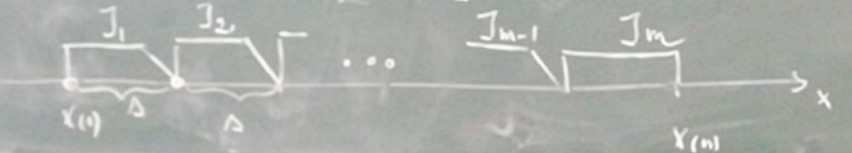
\includegraphics[scale=0.7]{5_1}}
\end{figure}

Определение интервального статистического ряда, отвечающего выборке $x$ называется таблица следующего вида:\\

\begin{figure}[H]
	\center{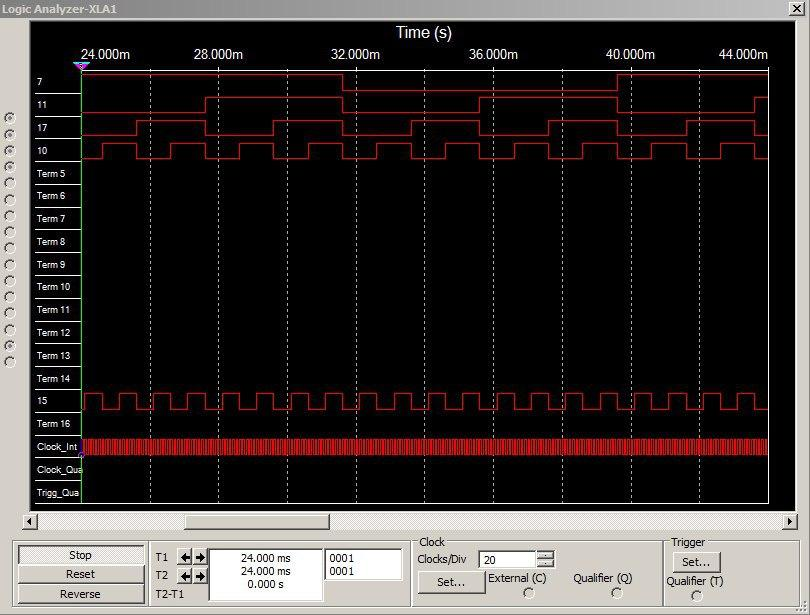
\includegraphics[scale=0.7]{5_2}}
\end{figure}

$n_{i}$ - число элементов выблоки $\overrightarrow{x}$, попавших в промежуток $J_{i}, i = \overline{1, m}$\\
Замечание:\\
1) $\sum\limits_{i = 1}^{m} n_{i} = n$\\
2) Для выбора m используют формулу:\\
$m = [log_{2}n] + 2$\\
или\\
$m = [log_{2}n] + 1$\\

\section{Эмпирическая плотность}
Пусть для данной выборки $\overrightarrow{x}$ построен интервальный статистический ряд $(J_{i}, n_{i}), i = \overline{1, m}$\\
Определение:\\
Эмпирической плотностью распределения соответствующей выборки $\overrightarrow{x}$ называется функция:\\
\begin{equation}
f_{n}(x) = 
\begin{cases}
\frac{n_{i}}{n \cdot \Delta}, x \in J_{i}\\
0
\end{cases}
\end{equation}

Замечание:
1) Очевидно, что $\int\limits_{-\infty}^{+\infty} f_{n} (x) dx = \int\limits_{x_{(1)}}^{x_{(m)}} f_{n} (x) dx = \sum\limits_{i=1}^{m}\frac{n_{i}}{n \cdot \Delta} \Delta = 1$\\
Таким образом эмпирическая плотность распределения удовлетворяет условию нормировки. Легко показать, что она обладает всеми свойствами функции плотности распределения.\\
2) $f_{n}(x)$ является кусочно-постоянной функцией:
\begin{figure}[H]
	\center{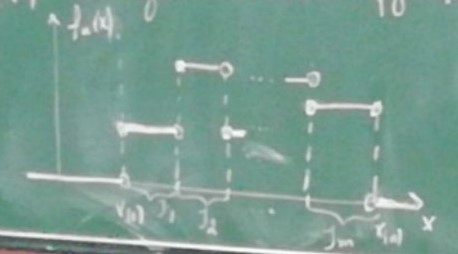
\includegraphics[scale=0.7]{5_3}}
\end{figure}

3) Функция $f_{n}(x)$ вяляется статистическим аналогом функции плотности распределения вероятности. Доказательство - аналогично доказанному выше результату для функции распределения. $\hat{F}_{n}(x) \overrightarrow{x \rightarrow \infty} F(x)$ на P\\

$f_{n}(x)$ примерно равна $f(x)$ при n >> 1.

Опредениение - график эмпирической функции плотности называется гистограммой.

\section{Полигон частот}
Определение полигона частот - пусть для некоторой выборки $\overrightarrow{x}$ построены гистограммы, по определению полигоном частот называется ломаная, звенья которой соединяют середины верних сторон соседних прямоугольников гистограммы.
\begin{figure}[H]
	\center{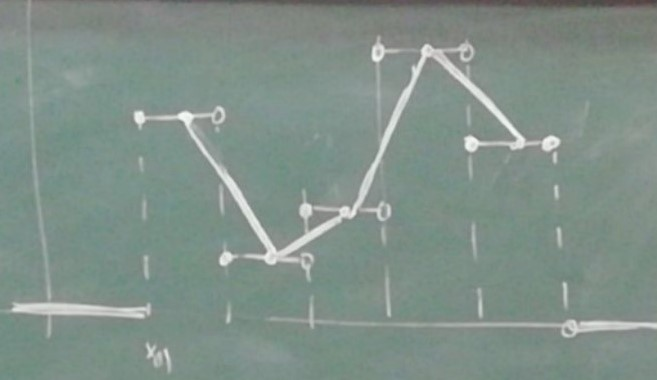
\includegraphics[scale=0.7]{5_4}}
\end{figure}

\section{Некоторые распределения, используемые в математической статистике}
\subsection{Гамма-функция Эйлера}
По определению гамма-функцией Эйлера называется выражение $\Gamma: R^{+} \rightarrow R$, определённое правилом:\\
$\Gamma(x) = \int\limits_{0}^{+\infty}e^{-t} t^{x-1}dt$\\

Замечание:\\
1) Интерграл является несобственным первого рода при $x \geqslant 1$;\\
при $x \in (0; 1)$ этот интеграл является несобственным и имеет следующие особенности: в t = 0 - подинтегральная функция имеет разрыв второго рода, верхний предел равен бесконечности. Легко проверить, что данный интеграл сходится при $x > 0$, при остальных вещественных x он расходится.\\

Некоторые свойства гамма-функции:\\
1. $\Gamma(x)$ - является бесконечное число раз дифференцируемой функцией, при этом её к-ая производная задаётся следующей формулой:\\
$\Gamma^{k}(x) = \int\limits_{0}^{+\infty} e^{-t} t^{x - 1} (ln t)^{k} dt$\\
2. $\Gamma(x + 1) = x\Gamma(x), x > 0$\\
3. $\Gamma(1) = 1$\\
4. $\Gamma(n + 1) = n!, n \in N$, по этой причине часто говорят, что гамма-функция является обобщением понятия факториала на вещественные числа.\\
5. $\Gamma(\frac{1}{2}) = \sqrt{\pi}$, вывод через интеграл Пуассона.
6. $\Gamma(\frac{n+1}{2}) = \bigg| $по второму свойству$\bigg| = \frac{n-1}{2}\Gamma(\frac{n-1}{2}) = ... = \frac{n-1}{2} \frac{n-2}{2} ...  \frac{1}{2} \Gamma(\frac{n-1}{2}) = \frac{1 \cdot 3 \cdot 5 ... \cdot (n - 1)}{2^{n}}\sqrt{\pi}$\\
7. Эскиз графика $\Gamma(x)$\\
\begin{figure}[H]
	\center{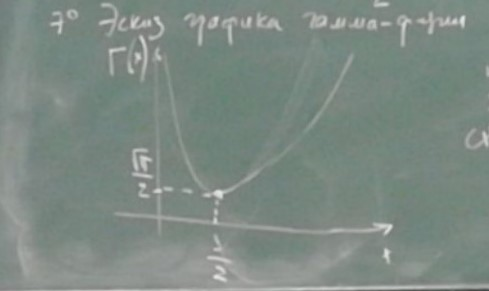
\includegraphics[scale=0.7]{5_5}}
\end{figure}

\subsection{Гамма-распределение}
Определение: говорят, что случайная величина $\xi$ имеет гамма-распределение, ели её функция плотности распределения вероятности имеет вид:\\
\begin{equation}
f_{\xi}(x) = 
\begin{cases}
\frac{\lambda^{\alpha}}{\Gamma(\alpha)} x^{\alpha - 1} e^{-\lambda x}, x  > 0\\

\end{cases}
\end{equation}
Обозначаеся как $\xi ~ \Gamma(\lambda, \alpha)$

Замечание:\\
1) Экспоненциальное распределениe:\\
\begin{equation}
f_{\xi}(x) = 
\begin{cases}
\lambda e^{-\lambda x}, x  > 0\\
0
\end{cases}
\end{equation}
$Exp(\lambda) = \Gamma(\lambda, 1)$\\

Теорема:\\
Пусть случайная величина $\xi_{1} ~ \Gamma(\lambda, \alpha_{1})$, а $\xi_{1} ~ \Gamma(\lambda, \alpha_{1})$, $\xi_{1}$ и $\xi_{2}$ - независимы. Тогда:\\
$\xi_{1} + \xi_{2} ~ \Gamma(\lambda, \alpha_{1} + \alpha_{2})$\\

Следствие:\\
Если случайные величины $\xi_{1}, \xi_{2}, ..., \xi_{n}$ независимы, причём $\xi_{i} ~ \Gamma(\lambda, \alpha_{i}), i = \overline{1, n}$, то:\\
$\xi_{1} + ... + \xi_{n} ~ \Gamma(\lambda, \alpha_{1} + ... + \alpha_{n})$\\

\subsection{Распределение Релея}
Пусть $\xi ~ \mathcal{N}(0, \sigma^{2})$\\
Говорят, что случайная величина $\xi$ имеет распределения Релея с параметром $\sigma$.

Замечание:\\
1) Несложно показать, что:\\
\begin{equation}
f_{y}(x) = 
\begin{cases}
\frac{1}{\sigma\sqrt{2\pi x}}e^{\frac{-x}{2b^{2}}}, x > 0\\
0
\end{cases}
\end{equation}

2) Распределение Релея является частным случаем гамма-распределения для $\lambda = \frac{1}{2\sigma^{2}}$ и $\lambda = \frac{1}{2}$, то есть $\nu ~ \Gamma(\frac{1}{2\sigma^{2}}, \frac{1}{2})$\\

\subsection{Распределение хи-квадрат}
Пусть:\\
Если случайные величины $\xi_{1}, \xi_{2}, ..., \xi_{n}$ независимы, $\xi_{i} ~ N(0, 1), i = \overline{1, n}$, $\nu = \xi_{1}^{2} + ... + \xi_{n}^{2}$\\

Определение: в этом случае говорят, что случайная величина $\nu$ имеет распределение хи-квадрат с n степенями свободы. Обозначается как $\nu ~ X^{2}(n)$\\

Замечание:\\
1)  $\xi_{i} ~ N(0, 1) \Rightarrow \xi^{2}_{i}$ имеет распределение Релея с параметром $\sigma = 1$, то есть $\xi^{2}_{i} ~ \Gamma(\frac{1}{2}, \frac{1}{2})$. Так как случайные величины $\xi_{1} ... \xi_{n}$ - независимы с учётом свойства гамма-распределения:\\
$\nu = \xi_{1}^{2} + ... + \xi^{2}_{n} ~ \Gamma(\frac{1}{2}, \frac{n}{2})$, то $X^{2} = \Gamma(\frac{1}{2}, \frac{n}{2})$\\
2) Очевидно, что если независимые случайные величины $\nu_{1}, ... \nu_{m}$ имеют распределения $X^{2} (\nu_{i} ~ X^{2} (k_{i}), i=\overline{1, m})$, то $\nu_{1} + ... + \nu_{n} ~ X^{2}(k_{1} + ... k_{m})$\\
3)График функции плотности $\nu ~ X^{2}(n)$\\
\begin{figure}[H]
	\center{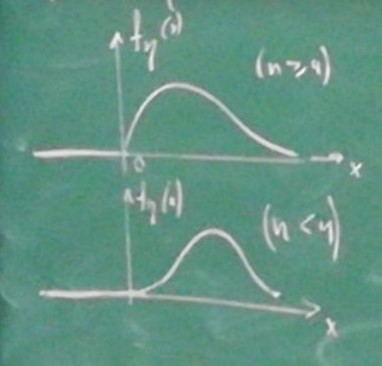
\includegraphics[scale=0.7]{5_6}}
\end{figure}

\subsection{Распределение Фишера}
Пусть:\\
1) $\xi_{1}, \xi_{2}$ - независимы
2) $\xi_{i} ~ X^{2}(n_{i}), i = \overline{1,2}$\\
3) $\nu = \frac{n_{1} \xi_{1}}{n_{2} \xi_{2}}$\\

Определение: в этом случае говорят, что случайная величина $\nu$ имеет распределение Фишера со степенями свободы $n_{1} и n_{2}$, $\nu ~ F(n_{1}, n_{2})$\\

Замечания:\\
1) Можно показать, что:\\
\begin{equation}
f_{\nu}(x) = 
\begin{cases}
C \frac{x^{\frac{n_{1}}{2} - 1}}{(1 + \frac{n_{1} x}{n_{2}})^{\frac{n_{1} + n_{2}}{2}}}, x > 0\\
0
\end{cases}
\end{equation}

$C = \frac{(\frac{n_{1}}{n_{2}})^{\frac{n_{1}}{2}}}{B(\frac{n_{1}}{2}, \frac{n_{2}}{2})}$\\
$B(x, y) = \int\limits_{0}^{1} t^{x - 1} (1 - t)^{y - 1} dt$  - бета-функция Эйлера.\\
2) Если $\nu ~ F(n_{1}, n_{2})$, то $\frac{1}{\nu} ~ F(n_{2}, n_{1})$\\








